\section{High-Speed-Logik}

\begin{itemize}
    \item Sättigung verhindern, da langsam (bei Bipolar-Transistoren)
    \item Reduzierter Spannungshub
    \item Stromsteuerung, da Ströme schneller geschaltet werden als Spannungen
\end{itemize}


\subsection{Emitter Coupled Logic (ECL)}

\begin{minipage}[c]{0.3\columnwidth}
    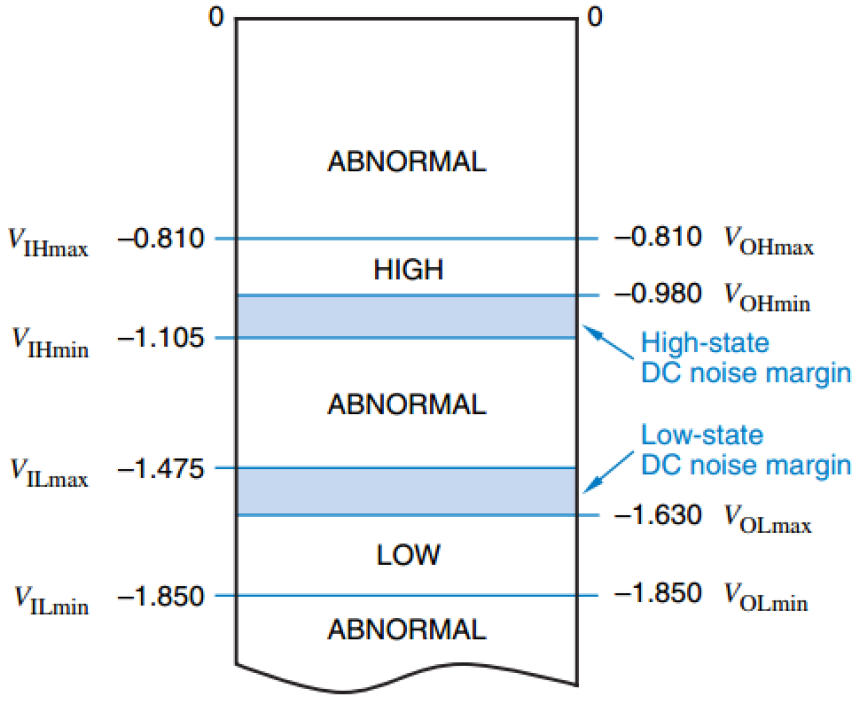
\includegraphics[width=\columnwidth]{images/ECL_logikpegel.png}
\end{minipage}
\hfill
\begin{minipage}[c]{0.68\columnwidth}
    \begin{itemize}
        \item 2 Familien: $10 \kilo$ (langsamer) und $100 \kilo$ (schneller)
        \item Positive Speisung: $V_{\rm CC} = 0 \, \volt$
        \item Negative Speisung: $V_{\rm EE} = -4.5 \, \volt$ / $V_{\rm EE} = -5.2 \, \volt$ 
        \item ICs werden warm ($40 \, \milli \watt$ pro Gatter)
    \end{itemize}
\end{minipage}

\begin{minipage}[c]{0.25\columnwidth}
    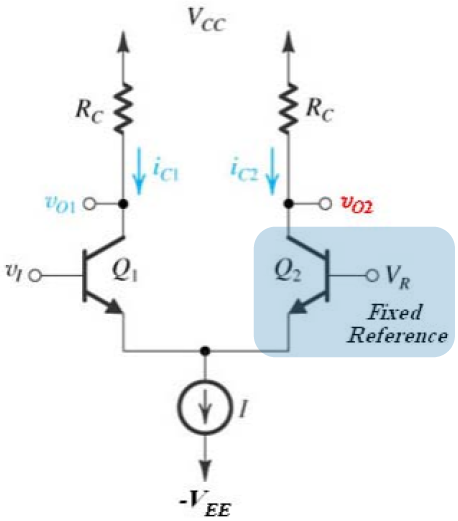
\includegraphics[width=\columnwidth]{images/ECL.png}
\end{minipage}
\hfill
\begin{minipage}[c]{0.72\columnwidth}
   \begin{itemize}
    \item Eingangssignal $V_{\rm I}$ wird mit fixer Referenz $V_{\rm R}$ verglichen
    \item Von $V_{\rm R} - 100 \, \milli \volt$ bis $V_{\rm R} + 100 \, \milli \volt$ \textbf{kippt Ausgangsspannung} von $V_{\rm CC}$ auf $V_{\rm CC} - R_{\rm C} \cdot I_{\rm C}$
    \item \textbf{Differentieller Spannungshub} der Ausgänge:\\ $V_{\rm diff} = \pm R_{\rm C} \cdot I_{\rm C}$
    \item Spannungspegel \textbf{nicht} kompatibel zu CMOS / TTL
   \end{itemize}
\end{minipage}


\subsubsection{Positive Emitter Coupled Logic PECL}

\begin{minipage}[c]{0.25\columnwidth}
    % Bild ist eventuell zu klein -> Testdruck machen
    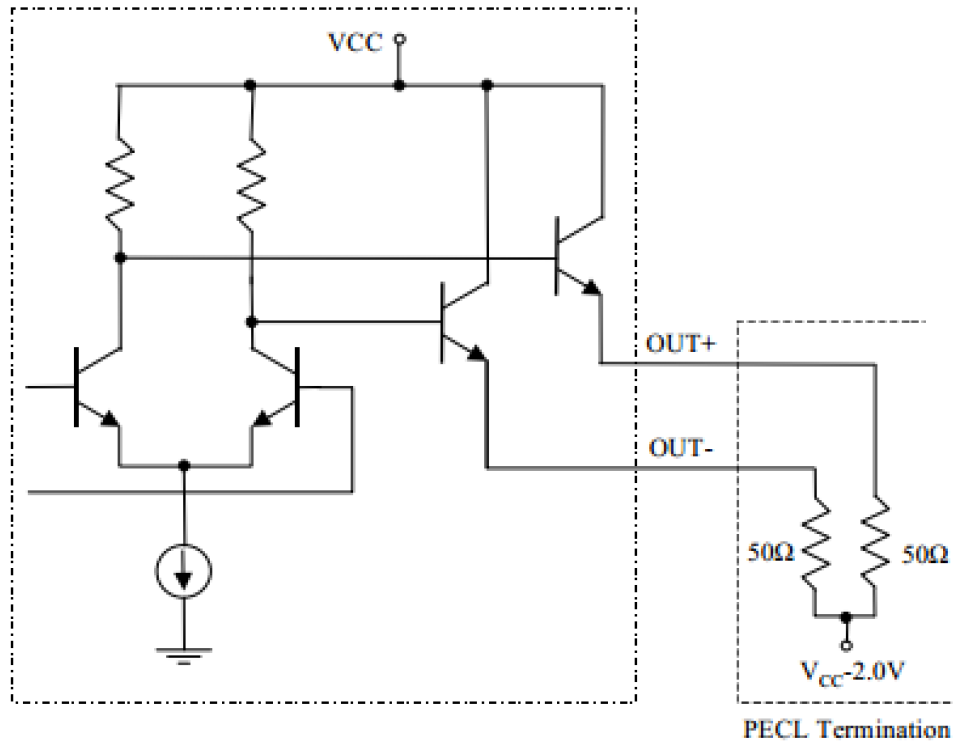
\includegraphics[width=\columnwidth]{images/PECL.png}
\end{minipage}
\hfill
\begin{minipage}[c]{0.72\columnwidth}
   \begin{itemize}
    \item Positive Speisung: $V_{\rm CC} = 5 \, \volt$
    \item Negative Speisung: $V_{\rm EE} = 0 \, \volt$
    \item Ausgangsbeschaltung mit $50 \, \ohm$ Abschluss zu $V_{\rm CC} - 2 \, \volt$ \\
        \textrightarrow\ Reduktion der Reflexionen!
    \item Spannungspegel sind kompatibel zu CMOS / TTL
   \end{itemize}
\end{minipage}

% falls zu wenig Platz, diese subsubsection weglassen
\subsubsection{Low Voltage Positive ECL (LVPECL)}

\begin{itemize}
    \item Speisespannungen:  $V_{\rm CC} = 3.3 \, \volt$; $V_{\rm EE} = 0 \, \volt$
    \item Weniger Leistung als $5 \, \volt$ Logik; leichter anpassbar an $3.3 \, \volt$ Logik
\end{itemize}


\subsection{Current Mode Logic (CML)}

\begin{minipage}[c]{0.25\columnwidth}
    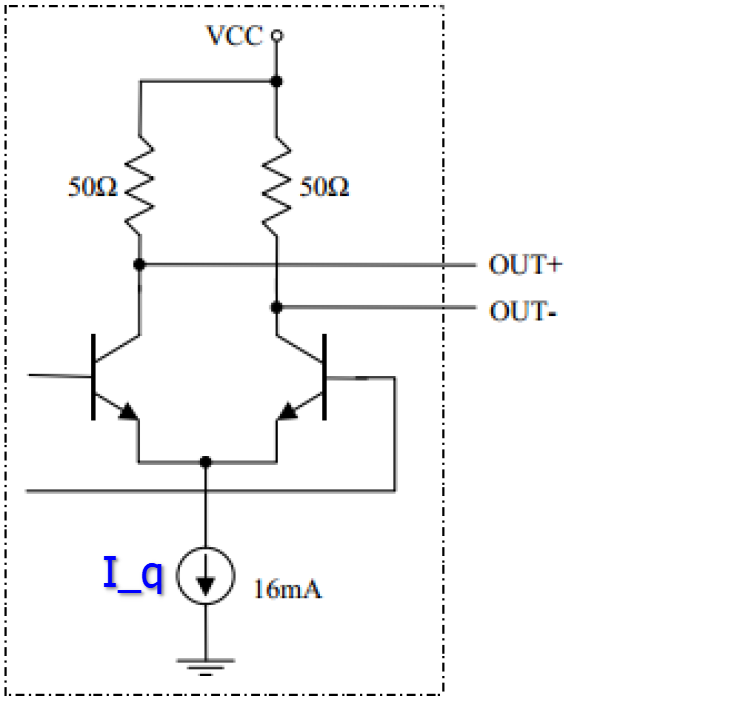
\includegraphics[width=\columnwidth]{images/CML.png}
\end{minipage}
\hfill
\begin{minipage}[c]{0.72\columnwidth}
   \begin{itemize}
    \item Terminierung am Eingang der Folgestufe gegen $V_{\rm CC}$
    \item Äquivalenter Widerstand: $R_{\rm C_{\rm eq}} = 50 \, \ohm \, || \, 50 \, \ohm = 25 \, \ohm$
    
    $$ \boxed{ \text{Differentielle Spannung: } V_{\rm diff} = \pm R_{\rm C_{\rm eq}} \cdot I_q }$$
   \end{itemize}
\end{minipage}


\subsubsection{CML vs. ECL}

\begin{minipage}[t]{0.55\columnwidth}
    \begin{center}
        \myul{\textbf{ECL}}
    \end{center}

    \begin{itemize}
        \item Diff-Amp mit Transistor-Buffer; Ausgang am Emitter 
        \item Single-ended Input (2. Eingang auf fixer Spannung)
        \item Single-ended Output (z.T. auch differentiell)
    \end{itemize}
\end{minipage}
\hfill
\begin{minipage}[t]{0.43\columnwidth}
    \begin{center}
        \myul{\textbf{CML}}
    \end{center}

    \begin{itemize}
        \item Ausgang direkt vom Diff-Amp
        \item Differentieller Input und differentieller Output
        \item Impedanzanpassung zur Reduktion von Reflexionen ($50 \, \ohm$)
    \end{itemize}
\end{minipage}


\subsubsection{Vorteile / Nachteile von CML gegenüber CMOS-Logik}

\begin{minipage}[t]{0.48\columnwidth}
    \raggedcolumns
    \begin{itemize}
        \item[+] high Speed
        \item[+] konstanter Strom (kaum Speisungseinbrüche)
        \item[+] differentiell: wenig Störung
        \item[+] kann Kabel treiben 
    \end{itemize}
\end{minipage}
\hfill
\begin{minipage}[t]{0.48\columnwidth}
    \raggedcolumns
    \begin{itemize}
        \item[-] hoher statischer Stromverbrauch
        \item[-] differentiell: benötigt doppelt so viele Leitungen
        \item[-] aufwändiges PCB-Layout wegen angepassten Leistungsimpedanzen nötig 
    \end{itemize}
\end{minipage}

